\documentclass[./main.tex]{subfiles}
\graphicspath{{\subfix{./Abbildungen/}}}
\begin{document}
\renewcommand{\tasktitle}{Sch*** OC}
\renewcommand{\taskpoints}{0}
\renewcommand{\taskweight}{5.8}
\aufgabenanfang
\blindtext

\begin{scheme}[H]
    \centering
        \schemestart[0, 1, thick]
            \chemfig{
                        % 1
                =^[:210]% 2
                 -[:270]% 3
                =^[:330]% 4
                  -[:30]% 5
                  ~[:90,,,,lmb]% 6
                 -[:150]% 1
            }
            \+{1.5em, 1.5em, -0.508cm}
            \chemfig{
                       % 1
               =_[:330]% 2
                -[:270]% 3
               =_[:210]% 4
            }
            \arrow{->}
            \chemfig{
                        % 1
                  -[:30]% 2
                 =^[:90]% 3
                           (
                     -[:150]% 4
                    =^[:210]% 5
                     -[:270]% 6
                    =^[:330]% -> 1
                           )
                  -[:30]% 7
                 -[:330]% 9
                =_[:270]% 10
                 -[:210]% 8
                           (
                     -[:150]% -> 2
                           )
            }
        \schemestop
    \caption{Ich bin eine Diels-Alder-Reaktion.}
    \label{sc:da_reaction}
\end{scheme}


Man kann auch ChemDraw-Dateien einf\"ugen. 
\begin{scheme}[H]
    \centering
    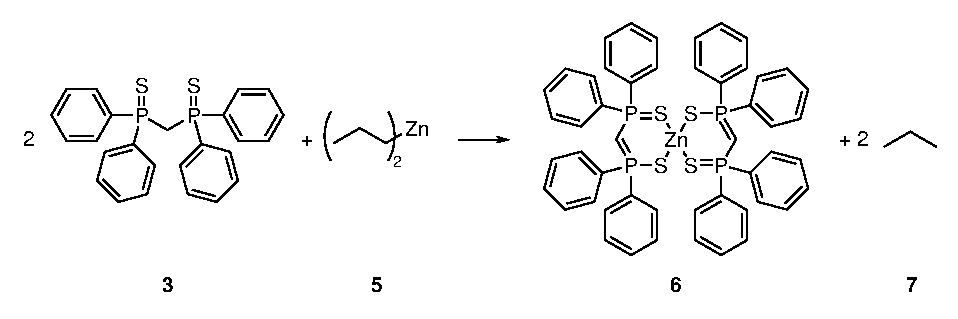
\includegraphics{Komplex.eps}
    \caption{Eine Synthese f\"ur die Tonne}
    \label{ACFKomplex}
\end{scheme}
Der Ligand wird wie folgt synthetisiert. 
\begin{scheme}[H]
    \centering
    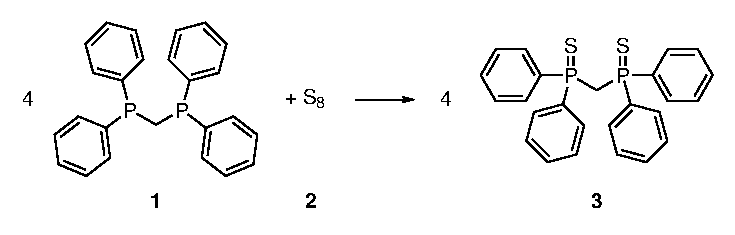
\includegraphics{Ligand.eps}
    \caption{Sehr komplizierte Synthese}
    \label{ACFLigand}
\end{scheme}
\begin{figure}[H]
    \centering
    
\includegraphics{IChO_2011_Logo_newblue.eps}
    \caption{Ein Bild im n\"achsten Kapitel.}
    \label{fig:my_label}
\end{figure}
\textcolor{orange}{Hier funktionierte der Seitenumbruch mit \textbackslash newpage nicht, solange nur das float-Objekt auf der Seite ist. Der Fall sollte irrelevant sein, da Aufgaben nie mir einem float-Objekt enden.}
\aufgabenende
\end{document}